\subsubsection{Ориентационные и зарядовые модели}

Все предложенные для объяснения фотоиндуцированной ГВГ модели можно разделить на два класса: ориентационные и зарядовые~\cite{dianov1995photoinduced}. 

\begin{figure}[h]
	\centering
	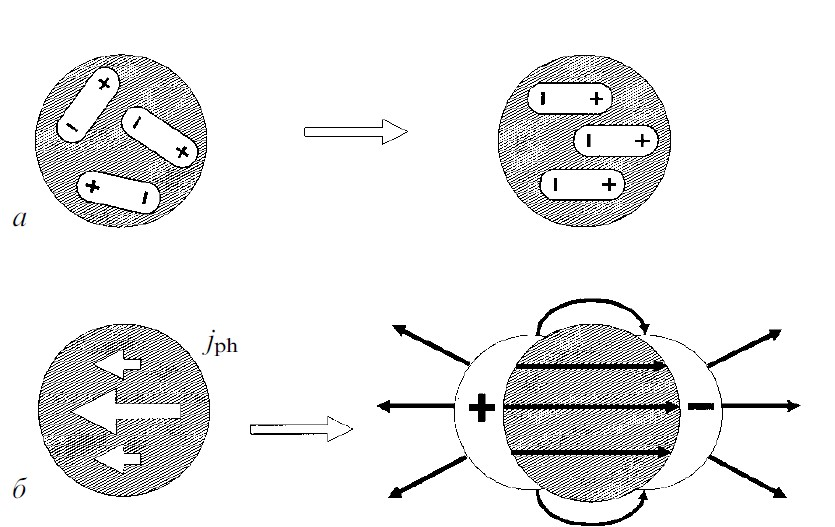
\includegraphics[width=0.55\linewidth]{Dissertation/images/review/models}
	\caption{Возникновение фотоиндуцированного электрического поля в ориентационных (а) и зарядовых (б) моделях}
	\label{fig:models}
\end{figure}


В ориентационных моделях (рис.~\cref{fig:models}, а)) предполагается, что асимметрия на микроскопическом уровне уже существует в виде хаотически ориентированных дипольных моментов (асимметричные молекулы, дефекты структуры). Под действием света происходит упорядочивание хаотически расположенных диполей:

\begin{equation}
	\mathbf{D} = \sum_i \mathbf{d}_i.
\end{equation}

В зарядовых моделях (рис.~\ref{fig:models}, б) предполагается, что под действием лазерного излучения происходит фотоионизация зарядов, макроскопическое их разделение и формирование постоянного электрического поля $E_{dc}$, которое через кубическую нелинейность индуцирует квадратичную восприимчивость:

\begin{equation}\label{eq:chi2_chi3}
	\chi^{(2)} = 3\chi^{(3)} E_{dc}.
\end{equation}

Важное отличие двух моделей заключается в характерных размерах области с ненулевым электрическим полем: в ориентационных моделях эта область сопоставима по размеру со световым пятном, в то время как в зарядовых моделях силовые линии электростатического поля простираются значительно дальше освещённой области (см.~\cref{fig:models}).

На основе накопленных экспериментальных данных были предложены две детальные микроскопические модели, объясняющие формирование решётки $\chi^{(2)}$: фотогальваническая модель Дианова и Стародубова~\cite{dianov1995photoinduced} и модель самоорганизации экситонов с переносом заряда Б.~Антонюка и В.~Антонюка~\cite{antonyuk2001self}. Обе модели относятся к классу зарядовых в том смысле, что связывают возникновение $\chi^{(2)}$ с наличием статического электрического поля $E_{dc}$. Однако они предлагают принципиально разные механизмы возникновения и усиления этого поля. Модель Антонюка, формально являясь ориентационной, включает положительную обратную связь, что принципиально отличает её от классических ориентационных моделей типа Столена--Тома. Ниже эти модели рассмотрены подробно, а затем приведены экспериментальные факты, которые каждая из них объясняет.
